\chapter{Requerimientos}
\label{cap:Requerimientos}

Éste capítulo detalla los requisitos de las aplicaciones, descritos como historias de usuario. Éstos señalan las necesidades de los clientes.

El cliente corresponde a miembros del equipo que lidera el proyecto FONDEF IDeA, código ID15I10560, proyecto orientado a generar herramientas para la gestión de desastres naturales. Los requerimientos se levantan en reuniones con los investigadores y responsables de aplicaciones del proyecto donde se estipulan las funcionalidades deseables, dichas reuniones tuvieron lugar en el Departamente de Ingeniería informática de la Universidad de Santiago e Chile.

\section{Proceso de toma de requerimientos}
\label{sec:tomaDeRequerimientos}

Dado que se seleccionó basarse, para el desarrollo de este proyecto, en la metodología \textit{Extreme Programming}, descrita en la sección \ref{subsec:MetodologiaDetalle} esta sección se detallará el proceso de toma de requerimientos basado en esta metodología, para ello se narra cómo se gestó el proyecto desde sus inicios y cómo se construyeron las Tabla \ref{tab:ReqTotalesC} y \ref{tab:ReqTotalesV}, presentadas en la sección \ref{sec:historias} correspondiente a las historias de usuario del sistema.

Inicialmente por parte del cliente, miembros del equipo del proyecto FONDEF IDeA, se tenía clara la visión del sistema en general, es decir, un sistema que haciendo uso de \textit{Twitter} detectara por medio de un sistema de procesamiento de \textit{streams} en tiempo real necesidades expresadas por la población en escenarios de catástrofe, mas no se tenía claro cómo éste debiese ser construido. 

Dado el caracter iterativo de la metodología, se definió el siguiente ciclo de operación entre el equipo de desarrollo — el autor del presente trabajo — y los clientes:

\begin{itemize}
\item Los días miércoles de cada semana, se realiza una reunión en la oficina de los clientes donde se muestran los resultados del trabajo de la semana anterior. Esto corresponde a una iteración.
\item En estas reuniones se entrega retroalimentación del trabajo realizado, señalando qué está bien y qué debiese ser modificado.
\item Se plantean nuevas funcionalidades deseables.
\item Al contrario de lo señalado por la metodología, no se realiza entrega del \textit{software} generado en estas iteraciones, pues lo que se espera es el \textit{software} final.
\end{itemize}

Las primeras cuatro iteraciones, correspondiente a las cuatro primeras semanas del proyecto, consistieron en \textit{spikes} de investigación para entender, entre otras cosas, el funcionamiento de \textit{Apache Storm}, procesamiento de información para ser categorizada, la captura de \textit{tweets} desde la API y las herramientas para el uso de mapas. 

Teniendo en consideración lo descrito anteriormente, ya desde el inicio se habían identificado algunas de las historias de usuario del sistema, estas eran: HU-c00, HU-c01, HU-v00, HU-v01 y HU-v03, correspondientes a su funcionamiento general y visualización.

El primer punto a ser construido la siguiente semana fue el apartado de comunicación (descrito en la sección \ref{sec:diseno:comunicacion}), para ello se generó la historia de usuario HU-c04 en la que se añadió un sistema de persitencia al sistema. A partir de aquí se esbozó la arquitectura del sistema descrita en la sección \ref{sec:Arquitectura}, que fue incorportando componentes a medida que se identificaron las demás historias de usuario.

Con respecto al apartado visual, habiendo presentado las historias de usuario HU-v00, como un prototipo de la intergaz, HU-v01, como marcadores dentro del mapa y HU-v03, como un refresco de las marcadores almacenados cada sierto tiempo se solicitaron nuevos elementos para mejorar la experiencia del usuario, así se dio origen a la historia HU-v06, la cual trata sobre la aplicación de iconos descriptivos a los marcadores de cada categoría. Además se solicitó que la configuación con respecto a la HU-v03 fuese automática, para ello se escribió una nueva historia de usuario: HU-v08.

La semana siguiente se solicitó que existieran diferentes formas de visualización de marcadores; se pidió que, segun el nivel de acercamiento del mapa, éstos se agruparan formando \textit{clusters} de marcadores que se agruparan según categoría dando origen a la historia HU-v02.

Producto de una charla realizada en la universidad donde se presentó una aplicación construida en la Universidad de Chile, referente a los efectos de desastres en redes sociales, se incorporó una nueva historia sobre una funcionalidad deseable para el sistema, la HU-v04, referente a la existencia de una línea de tiempo que mostrase la cantidad de eventos (necesidades), detectadas por fechas y que éstas pudiesen ser visualizadas en el mapa. Adicionalmente se señaló que era necesario un medio para que se incorporaran consultas al sistema, de manera de filtrar el flujo de datos de entrada según las necesidades de quien estuviese usando la aplicación, incorporando la HU-v05, además se señaló que se quería que el sistema mostrase estadísticas, sobre la actual consulta, referentes a la cantidad de eventos encontrados, procesados y usuarios, ésto se agregó en la HU-v07.

La siguiente iteración se solicitó la implementación de un método que extendiera la consulta realizada por el usuario (HU-v05), según los datos que se hubiesen obtenido hasta el momento, para ello se gestó la historia de usuario HU-c02.

Finalmente el cliente solicitó un módulo para actualizar el modelo de clasificación utilizado, inicialmente se pidió que éste fuese automático, pero ante la dificultad técnica de ello, dado que la entrada para el modelo debe ser ingresada por un usuario experto, se sugirío a los clientes realizar un cambio e implementar un actualizador manual del modelo del clasificador, lo cual fue aceptado y se registró como HU-c03.

Es importante señalar que la historia de usuario HU-c00, correspondiente a la detección de necesidades en sí corresponde a la historia más compleja del sistema y está compuesta por la construcción de múltiples operadores que pueden desarrollándose a lo largo del proyecto, por lo que no era posible completarla en una iteración. Lo que se realizó fue presentar avances en la construcción de operadores semanalmente.

\section{Historias de usuario y criterios de aceptación}
\label{sec:historias}

La sección \ref{sec:tomaDeRequerimientos} referenciaba, según lo descrito por la metodología \textit{extreme programming}, las historias de usuario correspondientes a lo que se requiere para el proyecto. Estas historias de usuario están plasmadas en las Tablas \ref{tab:ReqTotalesC} y \ref{tab:ReqTotalesV}, tienen la siguiente nomenclatura para su identificación: Aquellos que guarden relación con la aplicación de detección se identifican como 'HU-cXX', donde XX corresponde al número del requisito; 'HU-vYY' para aquellas que correspondan a la aplicación interfaz, donde, al igual que en el caso anterior, YY corresponden al número del requisito.

\begin{table}[H]
\centering
\caption[Resumen de las HU ligadas al procesamiento]{Resumen de las HU ligadas al procesamiento.\\Fuente: Elaboración Propia, (2016)}
\label{tab:ReqTotalesC}
\begin{tabular}{|c|l|}
\hline
\textbf{Identificador} & \multicolumn{1}{c|}{\textbf{Historia de usuario}} \\ \hline
HU-c00 & \begin{tabular}[c]{@{}l@{}}Como cliente quiero capturar necesidades de la población en tiempo real \\ cuando el país se encuentre en un escenario de catástrofe natural para\\ poder contar con información para asistir a la población afectada.\end{tabular} \\ \hline
HU-c01 & \begin{tabular}[c]{@{}l@{}}Como cliente quiero que las necesidades detectadas se recojan desde la \\ información generadas en redes sociales como Twitter, dado su caracter \\ informativo.\end{tabular} \\ \hline
HU-c02 & \begin{tabular}[c]{@{}l@{}}Como cliente quiero que la búsqueda de necesidades pueda ser extendida \\ automáticamente para encontrar información adicional que pueda ser de \\ apoyo.\end{tabular} \\ \hline
HU-c03 & \begin{tabular}[c]{@{}l@{}}Como usuario deseo poder incluir diferentes modelos de clasificación \\ dependiendo de las características del evento a analizar.\end{tabular} \\ \hline
HU-c04 & \begin{tabular}[c]{@{}l@{}}Como cliente quiero almacenar datos históricos para poder realizar \\ análisis mas a fondo, incluso entre diferentes eventos.\end{tabular} \\ \hline
\end{tabular}
\end{table}

\begin{table}[H]
\centering
\caption[Resumen de las HU ligadas a la interfaz]{Resumen de las HU ligadas a la interfaz.\\Fuente: Elaboración Propia, (2016)}
\label{tab:ReqTotalesV}
\begin{tabular}{|c|l|}
\hline
\textbf{Identificador} & \multicolumn{1}{c|}{\textbf{Historia de usuario}} \\ \hline
HU-v00 & \begin{tabular}[c]{@{}l@{}}Como usuario quiero una interfaz basada en un mapa geográfico donde\\ se pueda interactuar con la información generada.\end{tabular} \\ \hline
HU-v01 & \begin{tabular}[c]{@{}l@{}}Como cliente quiero que las necesidades detectadas puedan ser asociadas \\ aun punto en un mapa geográfico para poder identificar el lugar físico de \\ su fuente, esta ubicación debe ser de manera automática, incluso si no se \\ cuenta con los datos de geoubicación.\end{tabular} \\ \hline
HU-v02 & \begin{tabular}[c]{@{}l@{}}Como usuario quiero que puedan aplicarse filtros a la visualización de \\ los puntos de modo que según la distancia entre ellos, cuáles se quieran \\ mostrar y el nivel de acercamiento que tenga el mapa se entreguen \\ diferentes formas de mostrar la información para que la información se \\ visualice con facilidad.\end{tabular} \\ \hline
HU-v03 & \begin{tabular}[c]{@{}l@{}}Como usuario quiero que la visualización de eventos se realice en tiempo\\ real para tomar decisiones rápidas cuando la situación lo amerite.\end{tabular} \\ \hline
HU-v04 & \begin{tabular}[c]{@{}l@{}}Como usuario quiero visualizar eventos pasados, además quiero poder \\ seleccionar un intervalo de tiempo y que el sistema muestre todos los \\ eventos que se hayan detectado dentro de aquel intervalo de modo que \\ pueda realizarse una análisis a posteriori de la emergencia.\end{tabular} \\ \hline
HU-v05 & \begin{tabular}[c]{@{}l@{}}Como usuario quiero poder especificar términos de búsqueda para \\ acotar la búsqueda sólo a aquellos datos que contengan elementos\\ relevantes para la situación a analizar.\end{tabular} \\ \hline
HU-v06 & \begin{tabular}[c]{@{}l@{}}Como usuario quiero que cada punto, correspondiente a una necesidad \\ específica, tenga un diseño particular fácilmente identificable.\end{tabular} \\ \hline
HU-v07 & \begin{tabular}[c]{@{}l@{}}Como usuario quiero que sea posible visualizar estadísticas del \\ procesamiento de la aplicación por consulta.\end{tabular} \\ \hline
HU-v08 & \begin{tabular}[c]{@{}l@{}}Como usuario quiero poder modificar cuánto tiempo se visualizará un \\ evento antes de que sea considerado antiguo y cada cuánto tiempo se ha \\ de añadir la información de los nuevos eventos.\end{tabular} \\ \hline
\end{tabular}
\end{table}

Estas historias de usuario se corresponden con los criterios de aceptación descritos en las Tablas \ref{tab:criteriosAceptacionC} y \ref{tab:criteriosAceptacionV} que se presentan a continuación.

\begin{table}[H]
\centering
\caption[Criterios de aceptación para HU de procesamiento]{Criterios de aceptación para HU de procesamiento.\\Fuente: Elaboración Propia, (2016)}
\label{tab:criteriosAceptacionC}
\begin{tabular}{|l|l|}
\hline
\multicolumn{1}{|c|}{\textbf{Identificador}} & \multicolumn{1}{c|}{\textbf{Criterio de aceptación}} \\ \hline
HU-c00 & \begin{tabular}[c]{@{}l@{}}· Debe construirse una topologia para Storm capaz de detectar \\ las necesidades.\\ · Debe crearse un operador capaz de extraer información desde\\ una fuente de datos basada en texto.\\ · Debe almacenar informacion historica para una ventana de \\ tiempo definida por el usuario.\\ · Los elementos almacenados deben estar correctamente \\ etiquetados.\end{tabular} \\ \hline
HU-c01 & \begin{tabular}[c]{@{}l@{}}· Twitter debe ser desde donde se obtienen los datos de entrada \\ del sistema.\end{tabular} \\ \hline
HU-c02 & \begin{tabular}[c]{@{}l@{}}· Deben implementarse técnicas para realizar expansión de la \\ consulta.\end{tabular} \\ \hline
HU-c03 & · El modelo de clasificación debe poder modificarse. \\ \hline
HU-c04 & · Los datos deben estar almacenados en un repositorio local. \\ \hline
\end{tabular}
\end{table}

\begin{table}[]
\centering
\caption[Criterios de aceptación para HU de interfaz.]{Criterios de aceptación para HU de interfaz.\\Fuente: Elaboración Propia, (2016)}
\label{tab:criteriosAceptacionV}
\begin{tabular}{|l|l|}
\hline
\multicolumn{1}{|c|}{\textbf{Identificador}} & \multicolumn{1}{c|}{\textbf{Criterio de aceptación}} \\ \hline
HU-v00 & \begin{tabular}[c]{@{}l@{}}· Debe contarse con una interfaz que muestre los eventos \\ detectados por el sistema.\end{tabular} \\ \hline
HU-v01 & \begin{tabular}[c]{@{}l@{}}· El mapa de eventos debe mostrar los eventos, asociados a un \\ punto geográfico.\end{tabular} \\ \hline
HU-v02 & \begin{tabular}[c]{@{}l@{}}· Se debe poder filtrar por modos de agrupamiento.\\ · Se debe poder filtrar por categorías.\\ · El mapa debe permitir modificar su nivel de acercamiento.\end{tabular} \\ \hline
HU-v03 & · El mapa debe actualizarse automáticamente. \\ \hline
HU-v04 & \begin{tabular}[c]{@{}l@{}}· Debe poder seleccionarse el intervalo.\\ · Los eventos en el mapa deben modificarse según el intervalo \\ que se seleccione.\\ · Debe seleccionarse el intervalo mediante una línea de tiempo.\\ · Debe mostrarse un histograma con los eventos pasados \\ presentes en el sistema.\end{tabular} \\ \hline
HU-v05 & \begin{tabular}[c]{@{}l@{}}· Debe existir un lugar donde especificar éstos términos.\\ · El sistema debe mostrar qué términos se están utilizando para\\ la búsqueda actual.\end{tabular} \\ \hline
HU-v06 & \begin{tabular}[c]{@{}l@{}}· Cada evento de categorización diferente debe tener un icono \\ particular.\end{tabular} \\ \hline
HU-v07 & \begin{tabular}[c]{@{}l@{}}· Deben mostrarse la cantidad de usuarios diferentes que han \\ emitido estados detectados.\\ · Deben mostrarse la cantidad de necesidades detectadas.\\ · Deben mostrarse la cantidad de eventos procesados.\end{tabular} \\ \hline
HU-v08 & \begin{tabular}[c]{@{}l@{}}· Debe existir un lugar donde realizar el cambio de parámetros.\\ · Debe ser explícito el cambio de los parámetros de \\ funcionamiento en la interfaz.\end{tabular} \\ \hline
\end{tabular}
\end{table}

Estas historias fueron manejadas por el equipo de desarrollo como tarjetas dentro de un tablero Kanban, éste consiste en una pizarra, en este caso \textit{online}, donde se separa el trabajo por columnas. Se utilizaron cuatro columnas: 

\begin{itemize}
\item Por hacer: lista de todos las historias de usuario, divididas en tareas, que no se habían trabajado hasta ese punto del desarrollo.
\item Haciendo: lista de las tareas que estaban en siendo desarrolladas actualmente.
\item Por revisar: lista de las tareas finalizadas correspondientes a historias de usuario que no habían sido presentadas a los clientes aún.
\item Hecho: lista de las tareas finalizadas que ya hubieran sido presentadas a los clientes y no generaran nuevos cambios.
\end{itemize}

Se utilizó, además, un sistema de colores para las tarjetas del tablero, donde el color verde correspondía a elementos del módulo de visualización; y amarillo correspondía a elementos del módulo de procesamiento. Adicionalmente existía el color rojo, el cual acompañaba a uno de los anteriores para señalar un \textit{bug} en aquella tarea que debía ser corregido. 

La Figura \ref{fig:trello} presenta un ejemplo de lo anterior con la captura final del tablero Kanban realizado en la herramienta Trello.

\begin{figure}[H]
	\centering
	\captionsetup{justification=centering}
	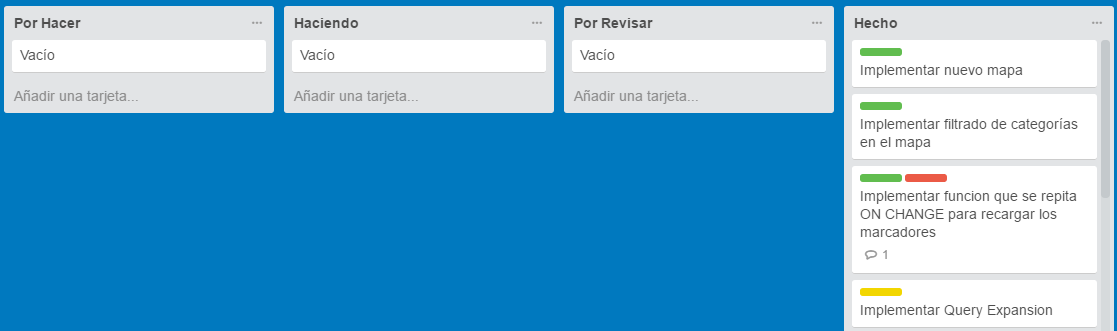
\includegraphics[scale=0.5]{images/Trello.png}
	\caption[Captura del estado final del tablero Kanban.]{Captura del estado final del tablero Kanban.\\Fuente: Elaboración Propia, (2016)}
	\label{fig:trello}
\end{figure}